\documentclass{article}
\usepackage[utf8]{inputenc}
\usepackage{enumitem}
\usepackage{enumerate}
\usepackage{amsmath}
\usepackage{graphicx}
\usepackage{subcaption}
\usepackage{natbib}
\usepackage{titlesec}

\titleformat{\section}
{\normalfont\Large\bfseries}{\thesection}{1em}{}[{\titlerule[0.8pt]}]

\title{ECON7103 HW3}
\author{Sedat Ors}
\date{February 5th}

\begin{document}

\maketitle

\section{Stata}

\begin{enumerate}
\item

\begin{itemize}
\item a)
\vspace{0.5cm}
Let's take the log of both sides
\begin{align}
y_i &= e^{\alpha} \delta^{d_i} z_i^{\gamma} e^{\eta_i} \\
\ln(y_i) &= \alpha \ln(e) + d_i \ln(\delta) + \gamma \ln(z_i) + \eta_i \ln(e) & \text{where} \quad \ln(e) = 1 \\
\ln(y_i) &= \alpha + d_i \ln(\delta) + \gamma \ln(z_i) + \eta_i
\end{align}
\vspace{0.5cm}

\item b)
$\delta$ means percentage change. if we increase $\delta$ 1 percent, ${y_i}$ changes 1 percent.  But if we need to interpret the retrofit program, it shows the effectiveness of the treatment program. if ${d_i} = $1 
it means everybody treated in the group if not $\delta$ =0. 
\vspace{0.5cm}

\item c)
when we take the derivative of the equation above according to the ${d_i}$,

\begin{align}
\Delta y_i &= y_i(d_i = 1) - y_i(d_i = 0)  \\
&= e^{\alpha\delta z_i^\gamma} e^{\eta_i} - e^{\alpha z_i^\gamma} e^{\eta_i} \\
&= (\delta - 1)e^{\alpha z_i^\gamma} e^{\eta_i} \\
\text{Multiply by } \frac{1}{y_i} = \frac{y_i}{y_i}: \\
&= \frac{(\delta - 1)e^{\alpha z_i^\gamma} e^{\eta_i} y_i}{e^{\alpha\delta d_i z_i^\gamma} e^{\eta_i}} \\
&= \frac{\delta - 1}{\delta d_i} y_i.
\end{align}

\item d)

\vspace{0.5cm}
Let's take the derivative of the equation above,




\begin{align}
\ln(y_i) &= \alpha + \ln(\delta)d_i + \gamma\ln(z_i) + \eta_i \\
y_i &= \exp\left(\alpha + \ln(\delta)d_i + \gamma\ln(z_i) + \eta_i\right)  \\
\frac{\partial y_i}{\partial z_i} &= \frac{\gamma}{z_i} \exp\left(\alpha + \ln(\delta)d_i + \gamma\ln(z_i) + \eta_i\right)
\end{align}

if we change ${z_i}$ 1 unit, ${y_i}$ change ${\gamma}{\frac{y_i}{z_i}}$
\vspace{0.5cm}

\item e)
\vspace{0.5cm}
\noindent See Table \ref{tab:HW3Q5}
\begin{table}[]
    \centering
     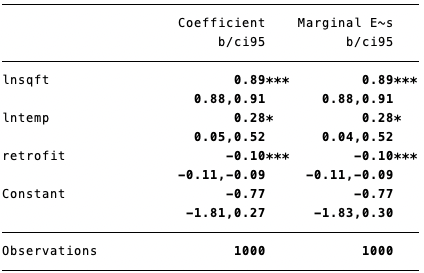
\includegraphics[]{HW3Q5.png}
    \caption{Electricity usage}
    \label{tab:HW3Q5}
\end{table}
\vspace{0.5cm}

\item f)
\vspace{0.5cm}
\noindent See Figure \ref{fig:HW3Q6} 
\begin{figure}[]
    \centering
     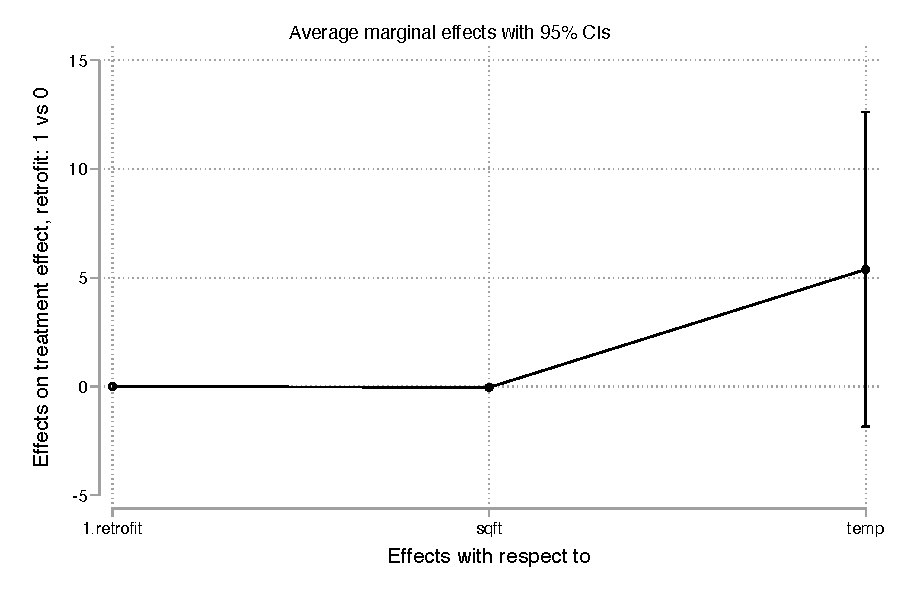
\includegraphics{HW3Q6.pdf}
    \caption{Marginal effects with 95\% confidence intervals}
    \label{fig:HW3Q6}
\end{figure}

\end {itemize}

\end{enumerate}

\end{document}

